\section{Results}

\subsection{Distinctiveness}

\begin{figure*}[t]
\centerline{% 
		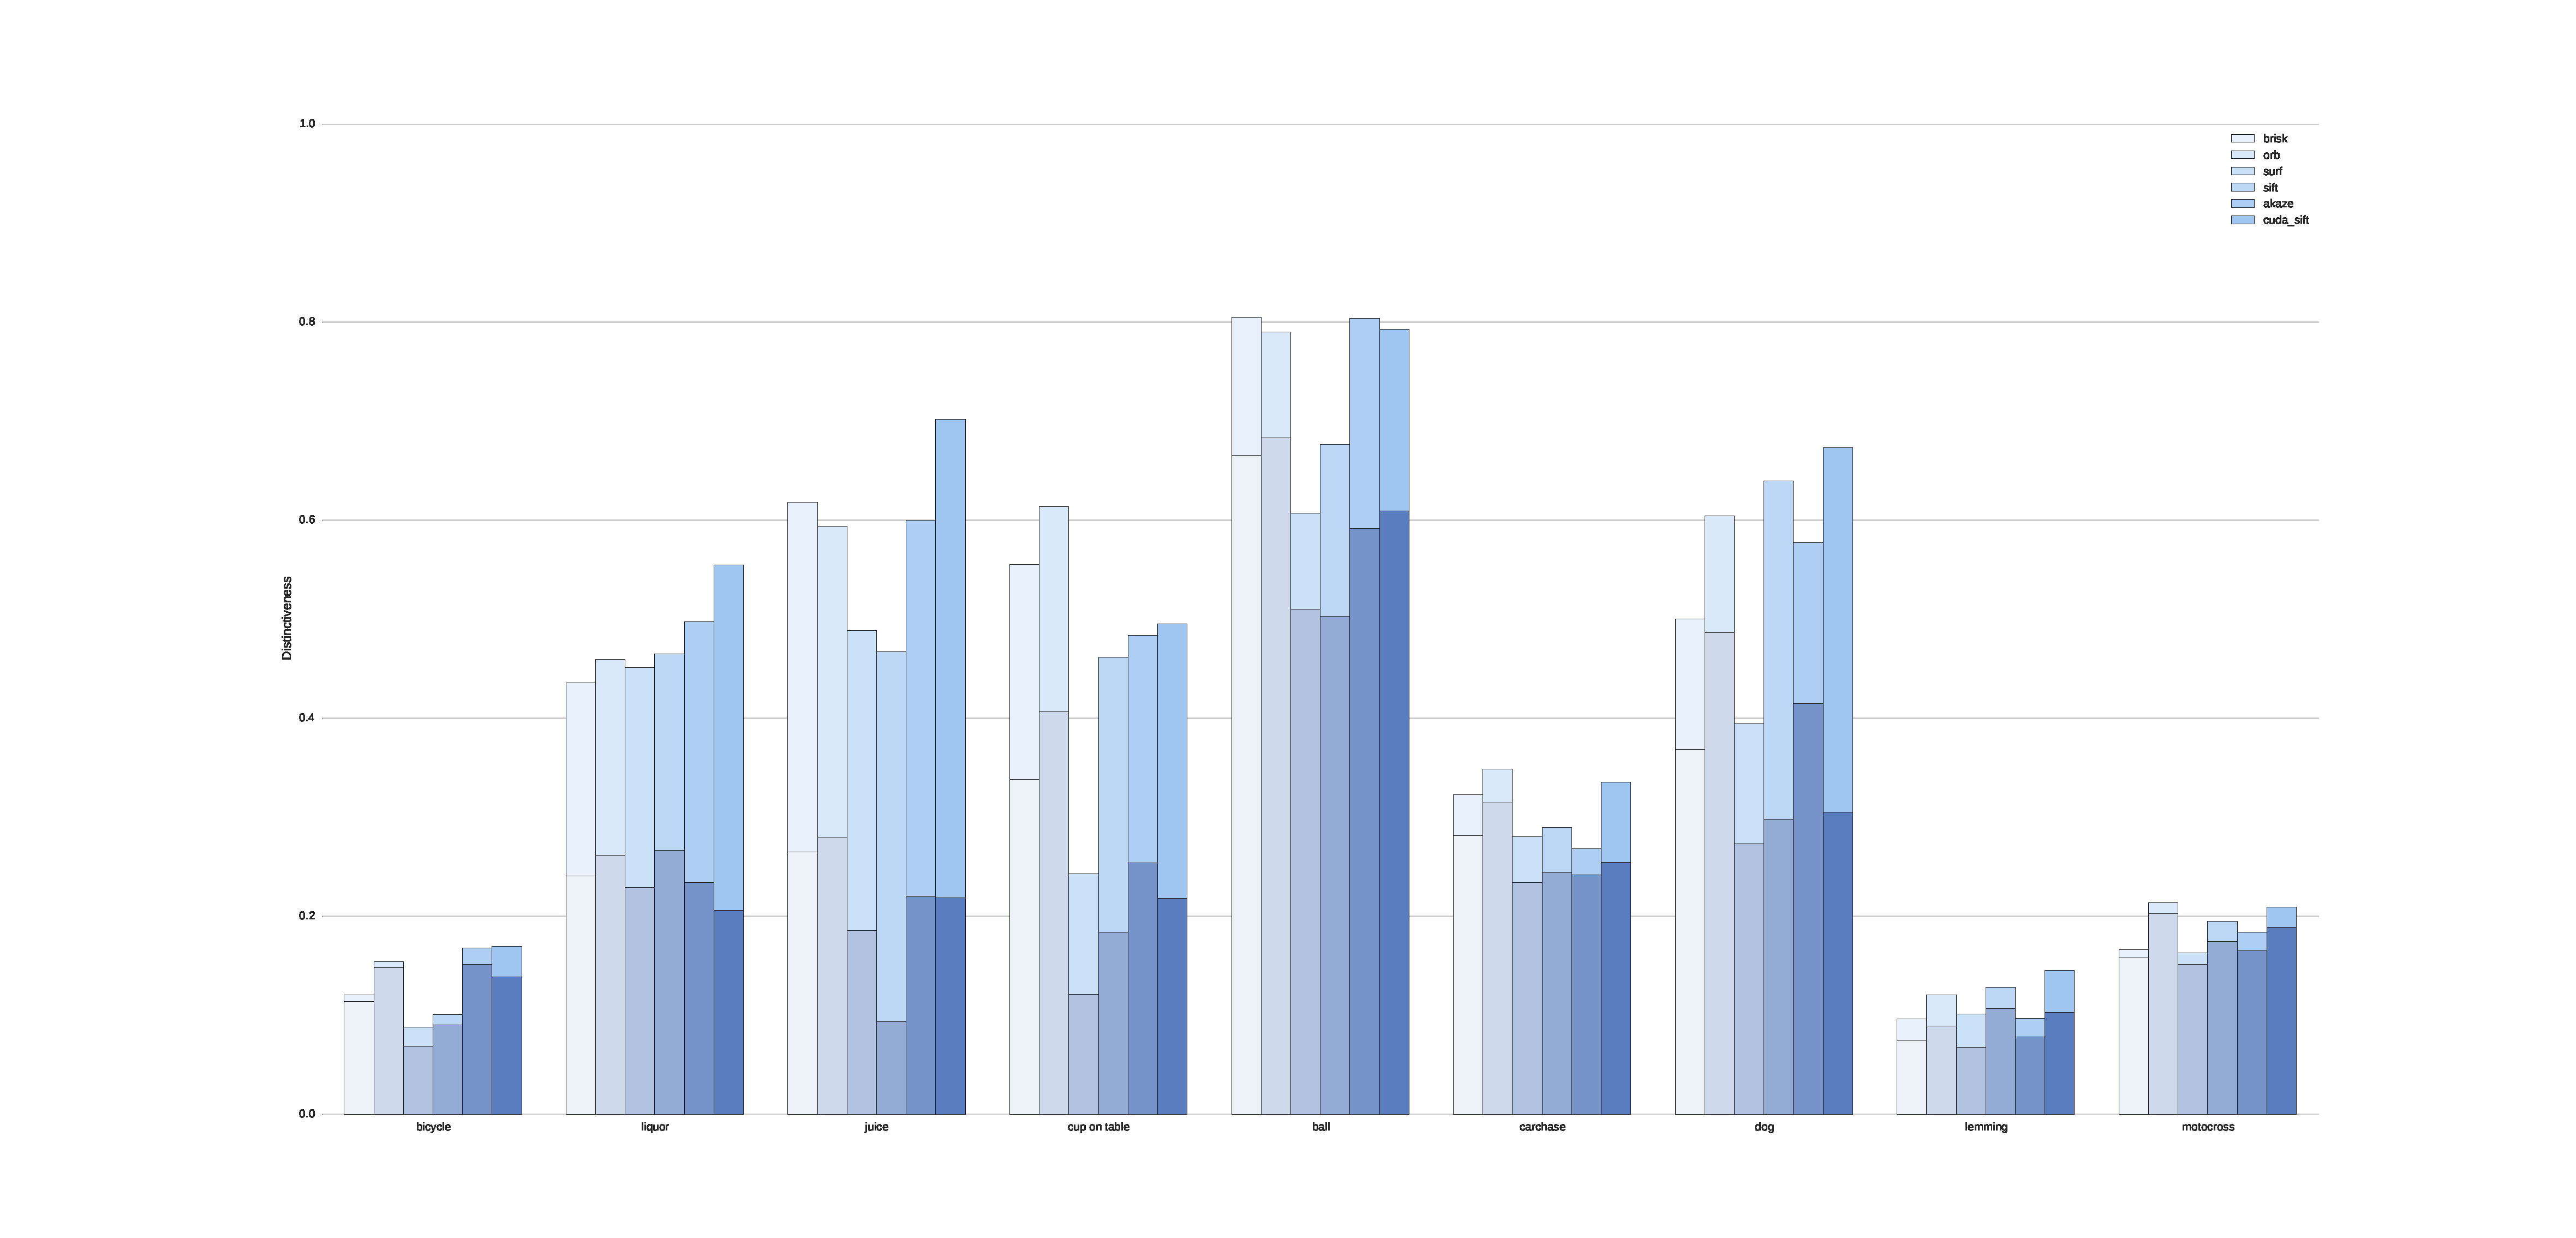
\includegraphics[width=0.98\linewidth]{imgs/distinctivenessTP.pdf}}
    \vspace{-2mm} 
	\caption{Examples take from the dataset showing the ratio of true positives and ambiguous true positives. The lighter color bars show the number of true positives that will actually pass the second best result test.}
	\label{fig:distinctiveness}
\end{figure*}

Fig.~\ref{fig:distinctiveness} shows the amount of true positives and ambiguous true positives for a subset of the videos present in the dataset. the lighter color bars show the number of descriptors that will pass the second best ratio filter. In Tab.~\ref{table:tp_ratio} shows the average ratios of effective true positives and total number of descriptors extracted on all the dataset. By effective true positive we intend all the positives matches that pass the second best match filter. Looking at the statistics it is interesting to notice that BRISK and ORB extract a higher number of feature descriptors in general and Fig.~\ref{fig:distinctiveness} shows that they have also a higher number of true positives, however if we calculate the number of true positives that pass the second best match check, then cuda SIFT and AKAZE have a better ratio of effective true positives. This is an indication that those descriptors are more distinctive. Upon inspection, the number of false positives is comparable as shown in Fig.~\ref{fig:false_positives}.

\begin{table}[h]
\centerline{% 
		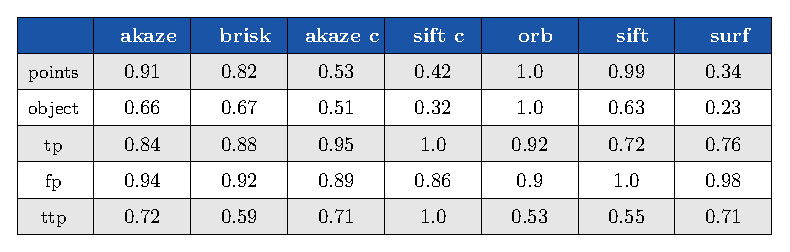
\includegraphics[width=0.98\linewidth]{tables/descriptivness_ratio.pdf}}
    \vspace{-2mm} 
	\caption{Average number of effective true positives and total feature extracted.}
	\label{table:tp_ratio}
\end{table}


\begin{figure}[t]
\centerline{% 
		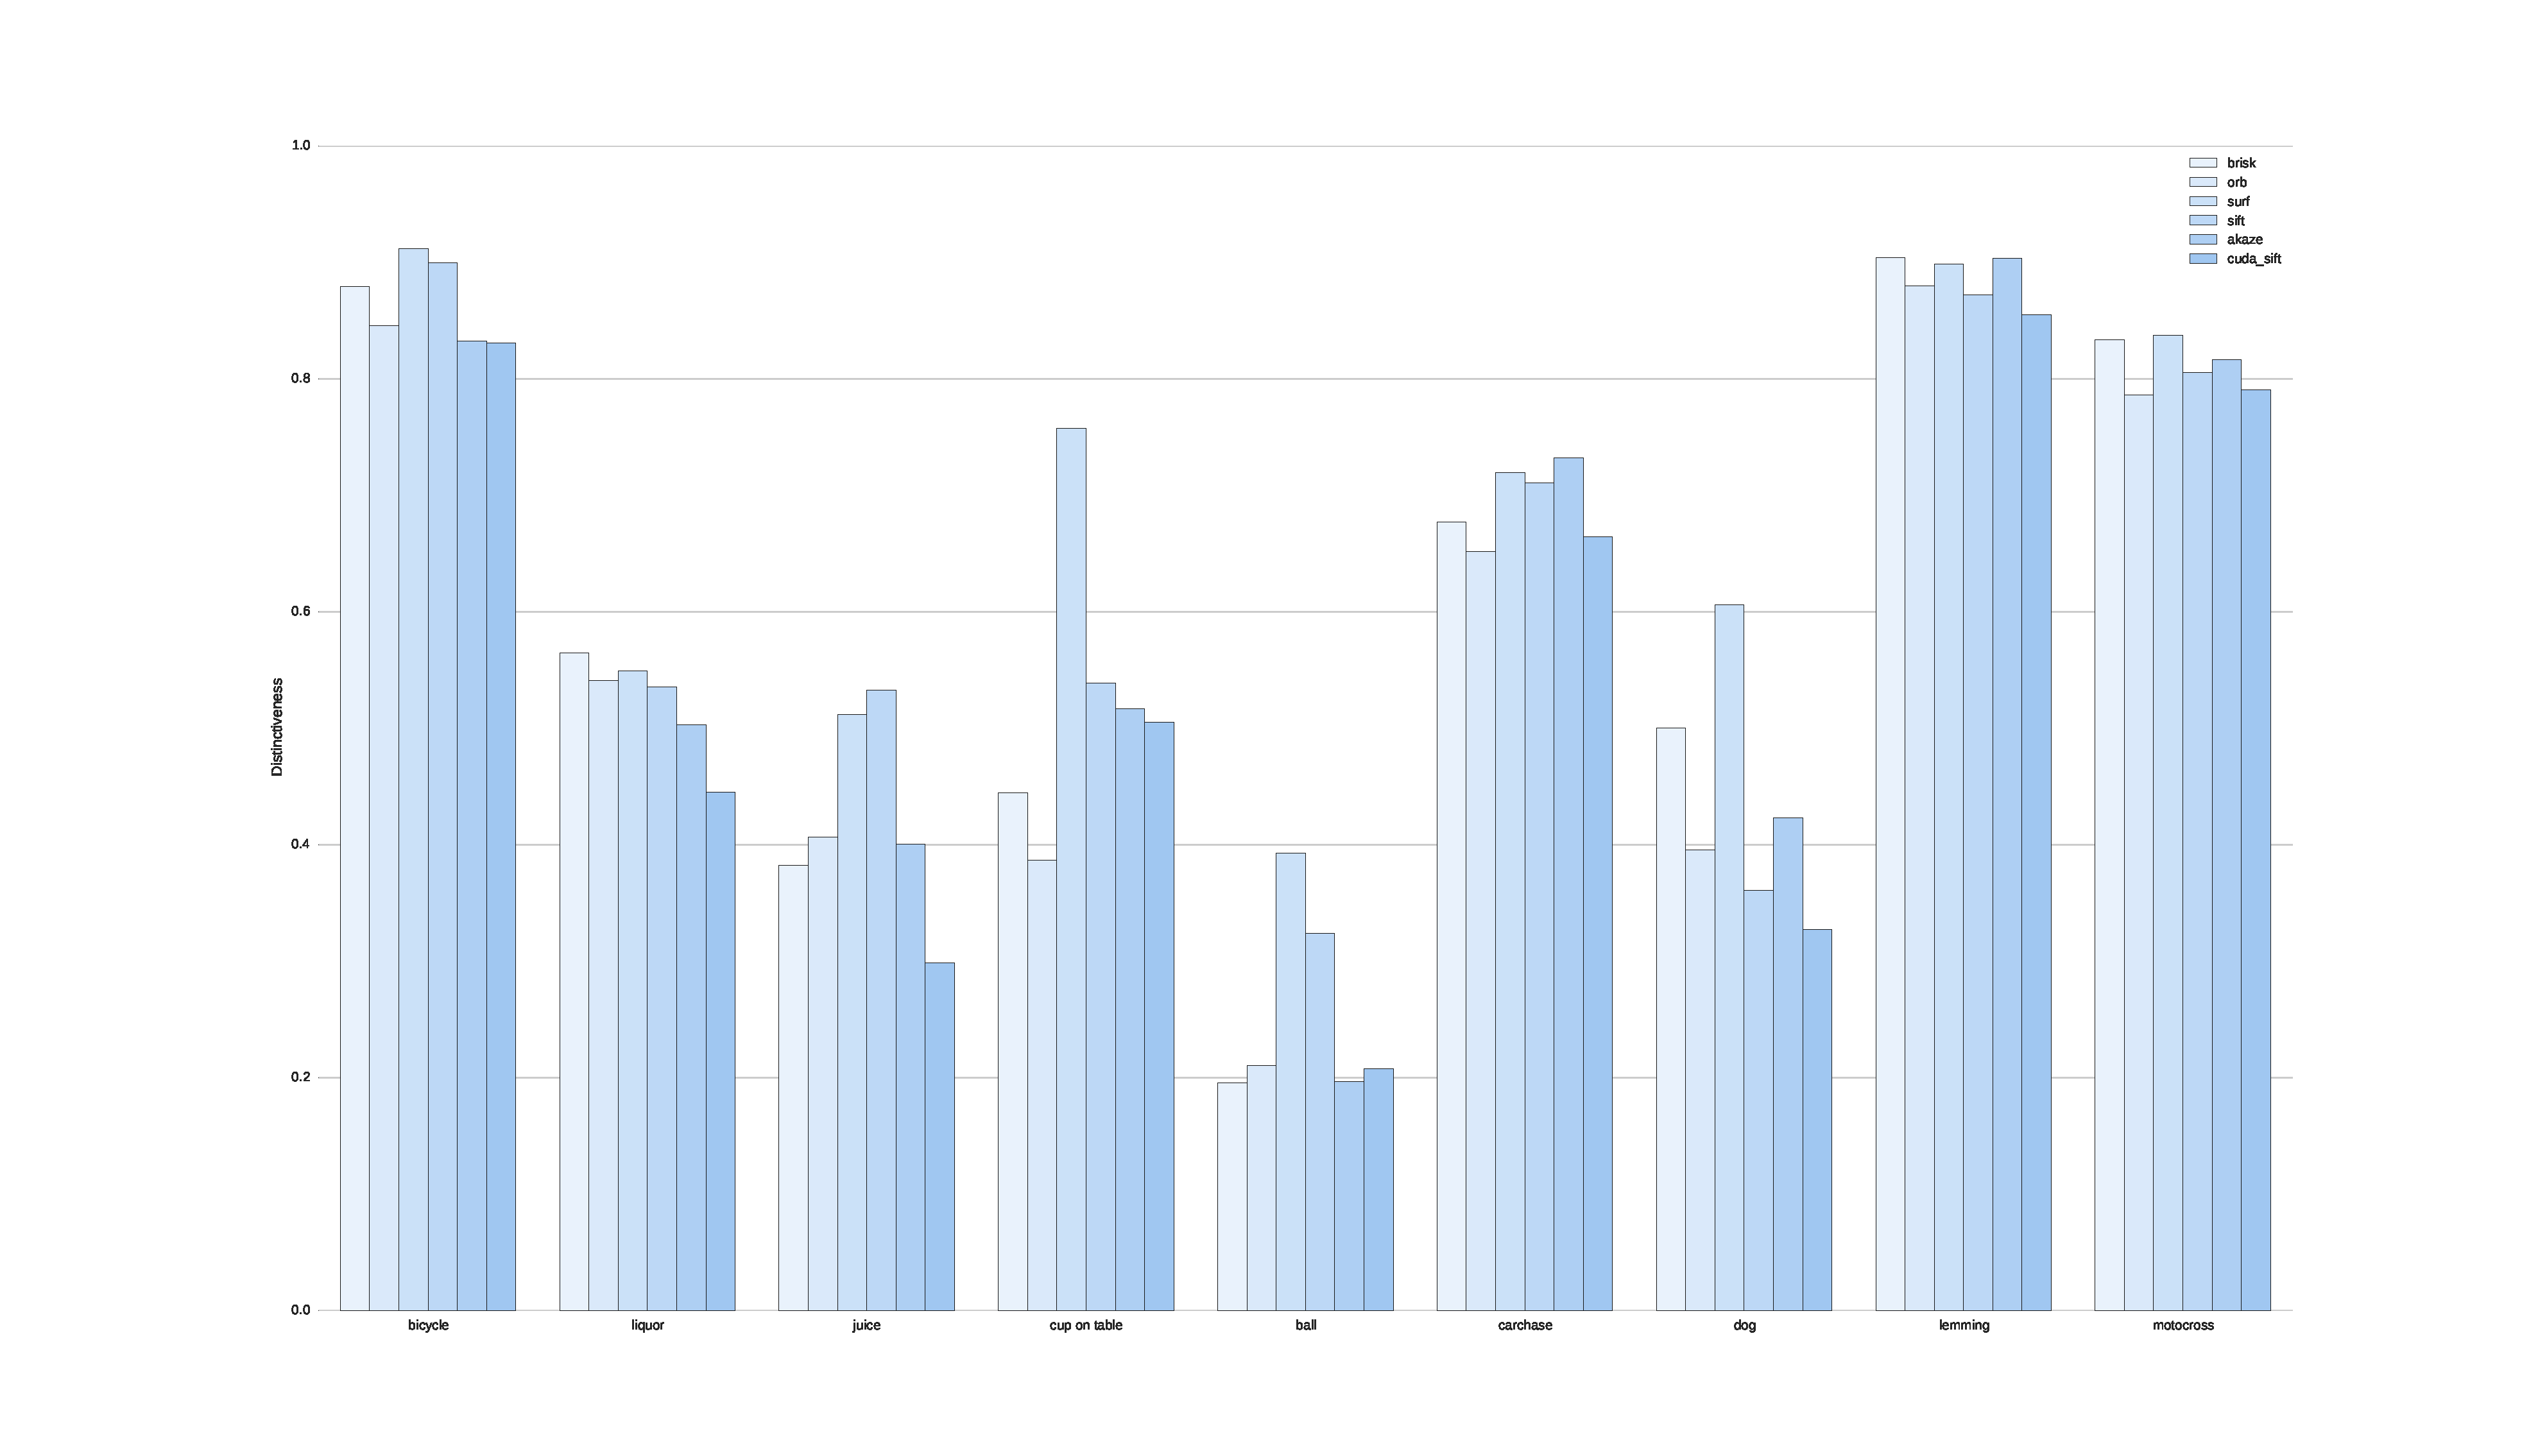
\includegraphics[width=0.98\linewidth]{imgs/false_positives.pdf}}
    \vspace{-2mm} 
	\caption{Examples take from the dataset showing the ratio of true positives and ambiguous true positives. The lighter color bars show the number of true positives that will actually pass the second best result test.}
	\label{fig:false_positives}
\end{figure}


\begin{figure*}[t]
\centerline{% 
		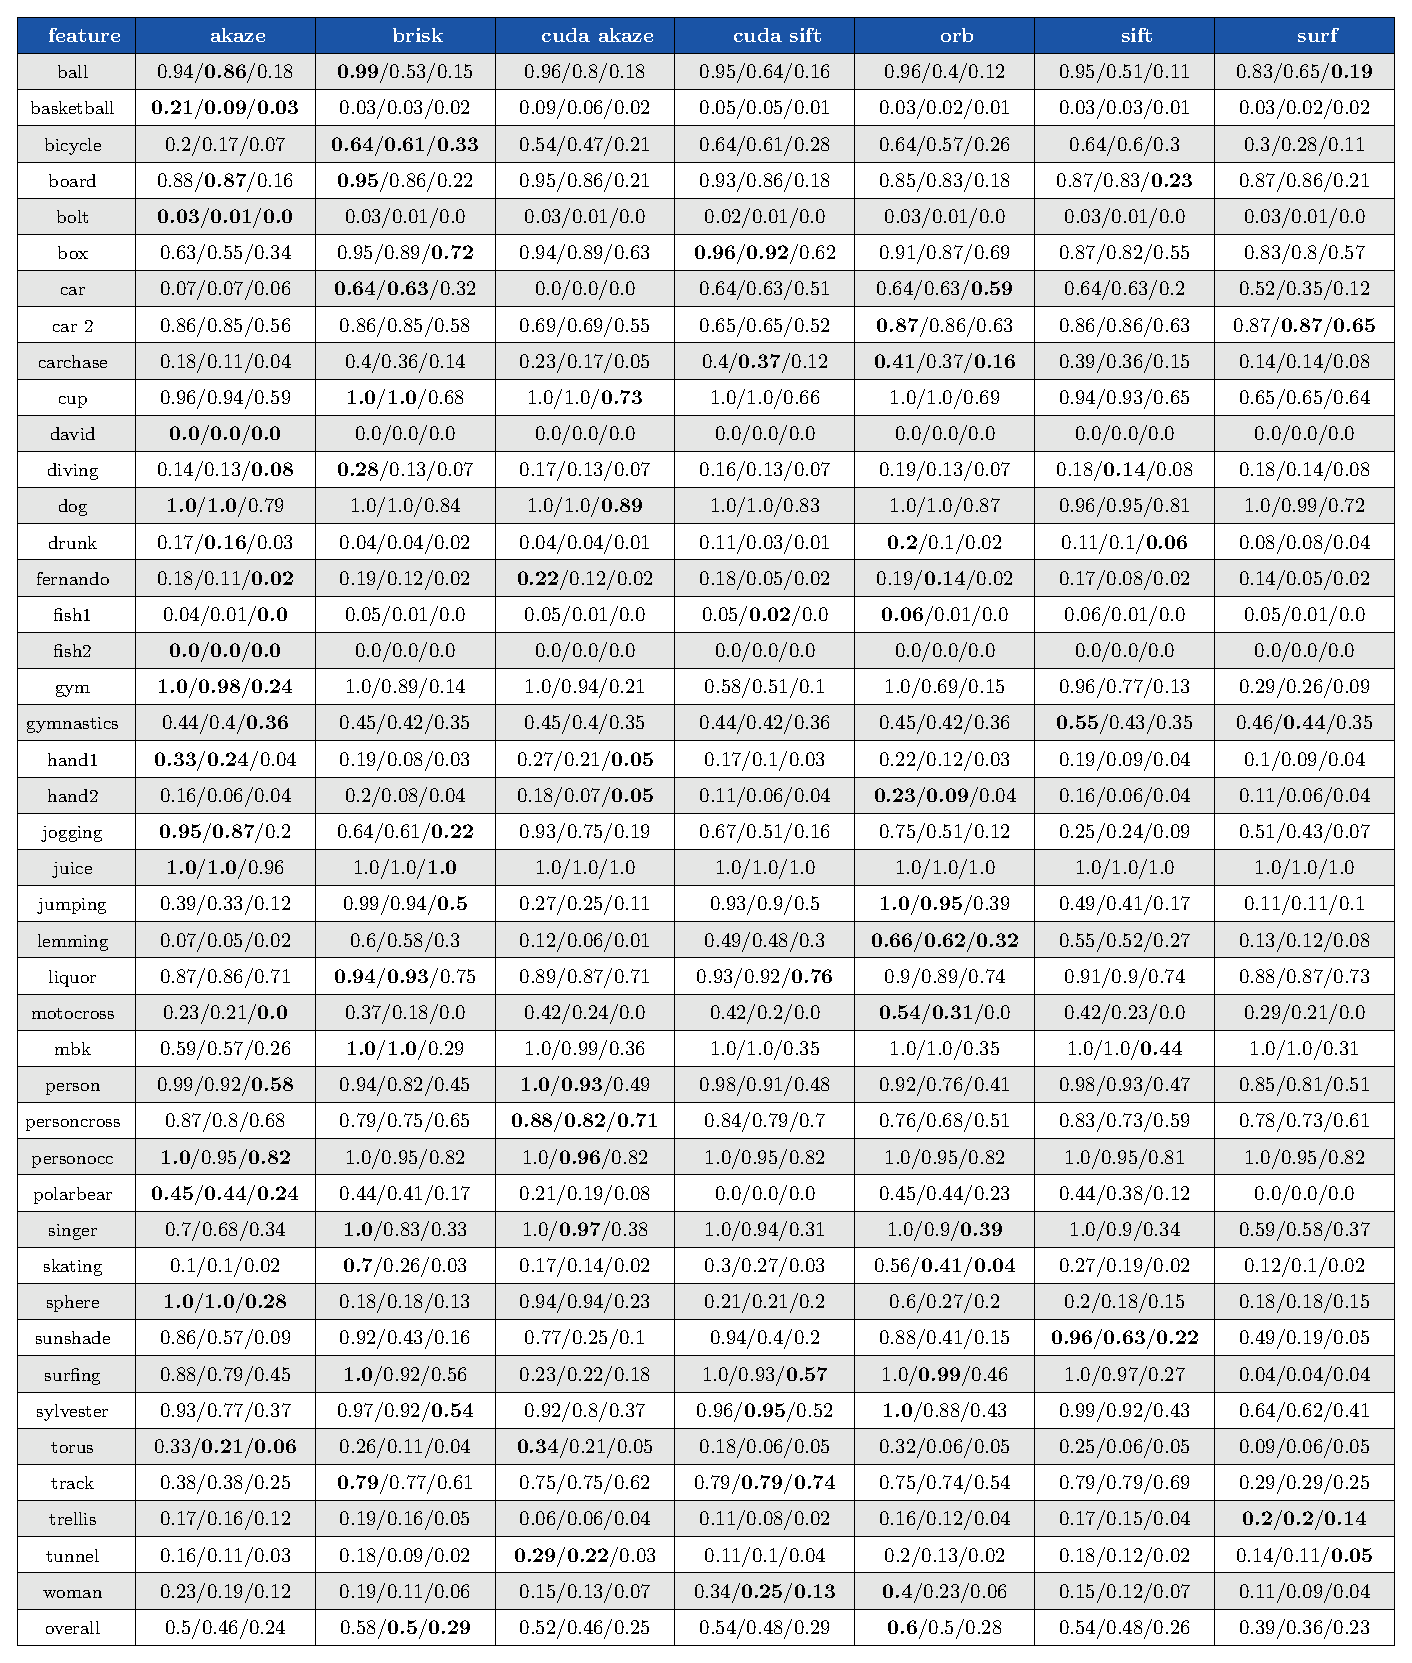
\includegraphics[width=0.98\linewidth]{tables/tracking_precision.pdf}}
    \vspace{-2mm} 
	\caption{Initial tracking results low,medium and high accuracy on all the dataset. Running new experiments on akaze right now with better parameters.}
	\label{fig:false_positives}
\end{figure*}